\documentclass[tikz, border=0mm, 12pt]{standalone}

\usetikzlibrary{arrows.meta,shadows,positioning,calc,decorations.markings}

\pgfdeclarelayer{timelines}
\pgfsetlayers{timelines,main}

\begin{document}

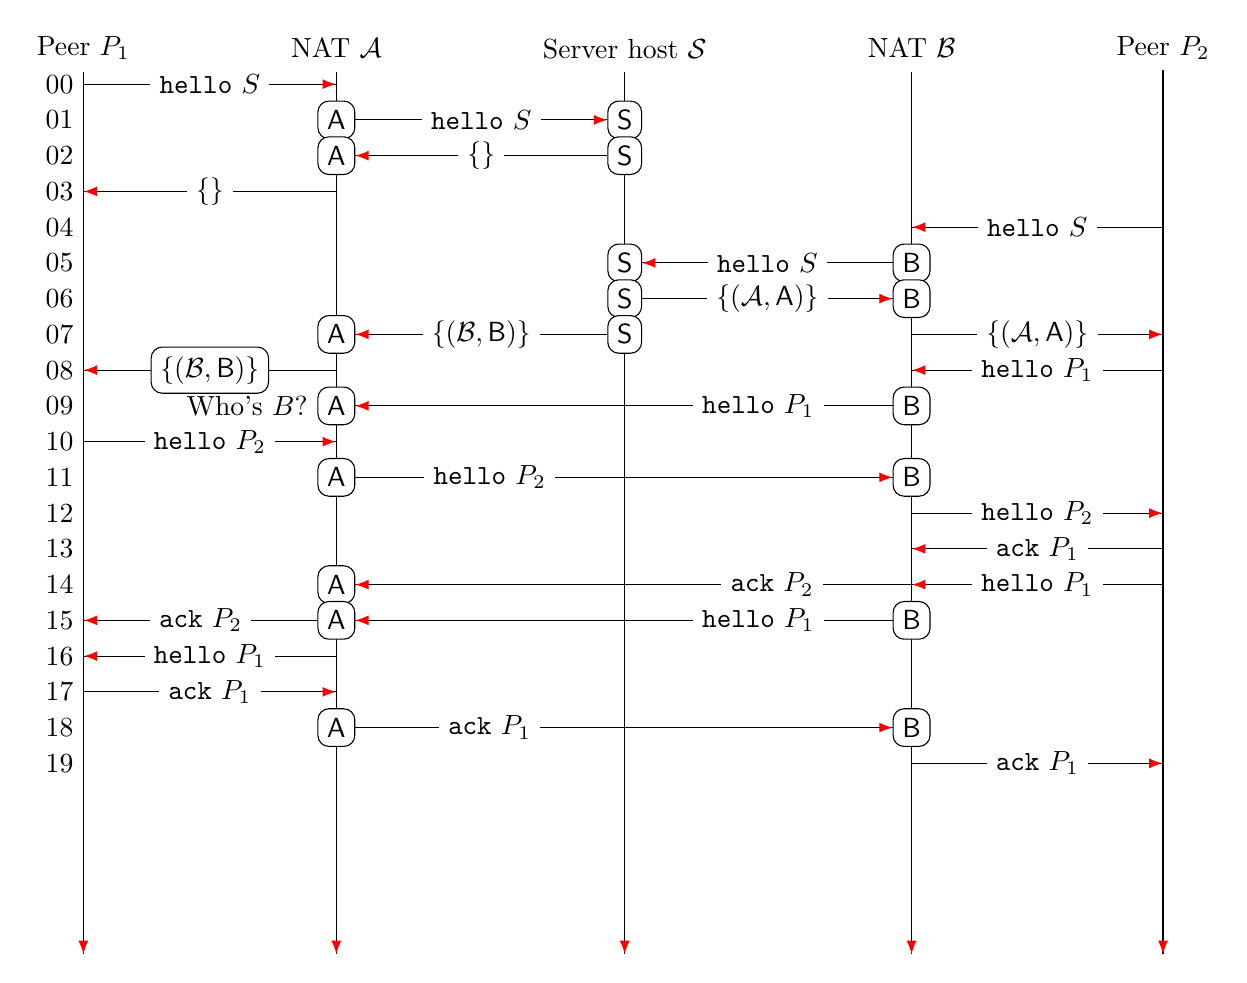
\begin{tikzpicture}
  
  \tikzset{myptr/.style={decoration={markings,mark=at position 1 with %
        {\arrow[red,scale=1.0,>=Latex]{>}}},postaction={decorate}}}
  
  % Entities
  \node[] (Peer A) {Peer $P_1$};
  \node[right=1.8 of Peer A] (NAT A) {NAT $\cal{A}$};
  \node[right=1.8 of NAT A] (Server) {Server host $\cal{S}$};
  \node[right=1.8 of Server] (NAT B) {NAT $\cal{B}$};
  \node[right=1.8 of NAT B] (Peer B) {Peer $P_2$};

  % Timelines
  \begin{pgfonlayer}{timelines}
    \coordinate (PA) at ($(Peer A.center) + (0.0,-11.5)$);
    \draw[myptr] ($(Peer A.center) + (0,-2ex)$) -- (PA);  
    \coordinate (NA) at ($(NAT A.center) + (0.0,-11.5)$);
    \draw[myptr] ($(NAT A.center) + (0,-2ex)$) -- (NA);
    \coordinate (S) at ($(Server.center) + (0.0,-11.5)$);
    \draw[myptr] ($(Server.center) + (0,-2ex)$) -- (S);
    \coordinate (NB) at ($(NAT B.center) + (0.0,-11.5)$);
    \draw[myptr] ($(NAT B.center) + (0,-2ex)$) -- (NB);
    \coordinate (PB) at ($(Peer B.center) + (0.0,-11.5)$);
    \draw[myptr] (Peer B) -- (PB);
  \end{pgfonlayer}
  
  % Time steps
  
  % 00
  \node (00) at ($(Peer A) + (-2ex,-3ex)$) {00};
  \node (PA00) at ($(Peer A) + (0,-3ex)$) [inner sep=0pt,minimum size=0pt] {};
  \path let \p{NAT A}=(NAT A),\p{00}=(00) in node (NA00) at (\x{NAT A},\y{00}) [inner sep=0pt,minimum size=0pt] {};
  \draw [myptr] (PA00) -- (NA00) node [pos=0.5,fill=white!100] {$\mathtt{hello}~S$};

  % 01
  \node (01) at ($(00) + (0,-3ex)$) {01};
  \path let \p{NAT A}=(NAT A),\p{01}=(01) in node (NA01) at (\x{NAT A},\y{01}) [fill=white!100,draw,rounded corners] {$\mathsf{A}$};
  \path let \p{Server}=(Server),\p{01}=(01) in node (S01) at (\x{Server},\y{01}) [fill=white!100,draw,rounded corners] {$\mathsf{S}$};
  \draw[myptr] (NA01) -- (S01) node [pos=0.5,fill=white!100] {$\mathtt{hello}~S$};

  % 02
  \node (02) at ($(01) + (0,-3ex)$) {02};
  \path let \p{Server}=(Server),\p{02}=(02) in node (S02) at (\x{Server},\y{02}) [fill=white!100,draw,rounded corners] {$\mathsf{S}$};
  \path let \p{NAT A}=(NAT A),\p{02}=(02) in node (NA02) at (\x{NAT A},\y{02}) [fill=white!100,draw,rounded corners] {$\mathsf{A}$};
  \draw[myptr] (S02) -- (NA02) node [pos=0.5,fill=white!100] {\{\}};

  % 03
  \node (03) at ($(02) + (0,-3ex)$) {03};
  \path let \p{NAT A}=(NAT A),\p{03}=(03) in node (NA03) at (\x{NAT A},\y{03}) [inner sep=0pt,minimum size=0pt] {};
  \path let \p{Peer A}=(Peer A),\p{03}=(03) in node (PA03) at (\x{Peer A},\y{03}) [inner sep=0pt,minimum size=0pt] {};
  \draw[myptr] (NA03) -- (PA03) node [pos=0.5,fill=white!100] {\{\}};

  % 04
  \node (04) at ($(03) + (0,-3ex)$) {04};
  \path let \p{Peer B}=(Peer B),\p{04}=(04) in node (PB04) at (\x{Peer B},\y{04}) [inner sep=0pt,minimum size=0pt] {};
  \path let \p{NAT B}=(NAT B),\p{04}=(04) in node (NB04) at (\x{NAT B},\y{04}) [inner sep=0pt,minimum size=0pt] {};
  \draw[myptr] (PB04) -- (NB04) node [pos=0.5,fill=white!100] {$\mathtt{hello}~S$};

  % 05
  \node (05) at ($(04) + (0,-3ex)$) {05};
  \path let \p{NAT B}=(NAT B),\p{05}=(05) in node (NB05) at (\x{NAT B},\y{05}) [fill=white!100,draw,rounded corners] {$\mathsf{B}$};
  \path let \p{Server}=(Server),\p{05}=(05) in node (S05) at (\x{Server},\y{05}) [fill=white!100,draw,rounded corners] {$\mathsf{S}$};
  \draw[myptr] (NB05) -- (S05) node [pos=0.5,fill=white!100] {$\mathtt{hello}~S$};

  % 06
  \node (06) at ($(05) + (0,-3ex)$) {06};
  \path let \p{Server}=(Server),\p{06}=(06) in node (S06) at (\x{Server},\y{06}) [fill=white!100,draw,rounded corners] {$\mathsf{S}$};
  \path let \p{NAT B}=(NAT B),\p{06}=(06) in node (NB06) at (\x{NAT B},\y{06}) [fill=white!100,draw,rounded corners] {$\mathsf{B}$};
  \draw[myptr] (S06) -- (NB06) node [pos=0.5,fill=white!100] {\{$(\cal{A},\mathsf{A})$\}};

  % 07
  \node (07) at ($(06) + (0,-3ex)$) {07};
  \path let \p{NAT B}=(NAT B),\p{07}=(07) in node (NB07) at (\x{NAT B},\y{07}) [inner sep=0pt,minimum size=0pt] {};
  \path let \p{Peer B}=(Peer B),\p{07}=(07) in node (PB07) at (\x{Peer B},\y{07}) [inner sep=0pt,minimum size=0pt] {};
  \draw[myptr] (NB07) -- (PB07) node [pos=0.5,fill=white!100] {\{$(\cal{A},\mathsf{A})$\}};
  \path let \p{Server}=(Server),\p{07}=(07) in node (S07) at (\x{Server},\y{07}) [fill=white!100,draw,rounded corners] {$\mathsf{S}$};
  \path let \p{NAT A}=(NAT A),\p{07}=(07) in node (NA07) at (\x{NAT A},\y{07}) [fill=white!10,draw,rounded corners] {$\mathsf{A}$};
  \draw[myptr] (S07) -- (NA07) node [pos=0.5,fill=white!100] {\{$(\cal{B},\mathsf{B})$\}};

  % 08
  \node (08) at ($(07) + (0,-3ex)$) {08};
  \path let \p{NAT A}=(NAT A),\p{08}=(08) in node (NA08) at (\x{NAT A},\y{08}) [inner sep=0pt,minimum size=0pt] {};
  \path let \p{Peer A}=(Peer A),\p{08}=(08) in node (PA08) at (\x{Peer A},\y{08}) [inner sep=0pt,minimum size=0pt] {};
  \draw[myptr] (NA08) -- (PA08) node [pos=0.5,fill=white!100,draw,rounded corners] {\{$(\cal{B},\mathsf{B})$\}};
  \path let \p{NAT B}=(NAT B),\p{08}=(08) in node (NB08) at (\x{NAT B},\y{08}) [inner sep=0pt,minimum size=0pt] {};
  \path let \p{Peer B}=(Peer B),\p{08}=(08) in node (PB08) at (\x{Peer B},\y{08}) [inner sep=0pt,minimum size=0pt] {};
  \draw[myptr] (PB08) -- (NB08) node [pos=0.5,fill=white!100] {$\mathtt{hello}~P_1$};

  % 09
  \node (09) at ($(08) + (0,-3ex)$) {09};
  \path let \p{NAT B}=(NAT B),\p{09}=(09) in node (NB09) at (\x{NAT B},\y{09}) [fill=white!100,draw,rounded corners] {$\mathsf{B}$};
  \path let \p{NAT A}=(NAT A),\p{09}=(09) in node (NA09) at (\x{NAT A},\y{09}) [fill=white!100,draw,rounded corners] {$\mathsf{A}$};
  \draw [myptr] (NB09) -- (NA09) node [pos=0.25,fill=white!100] {$\mathtt{hello}~P_1$};
  \node [left=0 of NA09] {Who's $B$?};

  % 10
  \node (10) at ($(09) + (0,-3ex)$) {10};
  \path let \p{Peer A}=(Peer A),\p{10}=(10) in node (PA10) at (\x{Peer A},\y{10}) [inner sep=0pt,minimum size=0pt] {};
  \path let \p{NAT A}=(NAT A),\p{10}=(10) in node (NA10) at (\x{NAT A},\y{10}) [inner sep=0pt,minimum size=0pt] {};
  \draw [myptr] (PA10) -- (NA10) node [pos=0.5,fill=white!100] {$\mathtt{hello}~P_2$};

  % 11
  \node (11) at ($(10) + (0,-3ex)$) {11};
  \path let \p{NAT A}=(NAT A),\p{11}=(11) in node (NA11) at (\x{NAT A},\y{11}) [fill=white!100,draw,rounded corners] {$\mathsf{A}$};
  \path let \p{NAT B}=(NAT B),\p{11}=(11) in node (NB11) at (\x{NAT B},\y{11}) [fill=white!100,draw,rounded corners] {$\mathsf{B}$};
  \draw [myptr] (NA11) -- (NB11) node [pos=0.25,fill=white!100] {$\mathtt{hello}~P_2$};

  % 12
  \node (12) at ($(11) + (0,-3ex)$) {12};
  \path let \p{NAT B}=(NAT B),\p{12}=(12) in node (NB12) at (\x{NAT B},\y{12}) [inner sep=0pt,minimum size=0pt] {};
  \path let \p{Peer B}=(Peer B),\p{12}=(12) in node (PB12) at (\x{Peer B},\y{12}) [inner sep=0pt,minimum size=0pt] {};
  \draw[myptr] (NB12) -- (PB12) node [pos=0.5,fill=white!100] {$\mathtt{hello}~P_2$};

  % 13
  \node (13) at ($(12) + (0,-3ex)$) {13};
  \path let \p{Peer B}=(Peer B),\p{13}=(13) in node (PB13) at (\x{Peer B},\y{13}) [inner sep=0pt,minimum size=0pt] {};
  \path let \p{NAT B}=(NAT B),\p{13}=(13) in node (NB13) at (\x{NAT B},\y{13}) [inner sep=0pt,minimum size=0pt] {};
  \draw[myptr] (PB13) -- (NB13) node [pos=0.5,fill=white!100] {$\mathtt{ack}~P_1$};

  % 14
  \node (14) at ($(13) + (0,-3ex)$) {14};
  \path let \p{Peer B}=(Peer B),\p{14}=(14) in node (PB14) at (\x{Peer B},\y{14}) [inner sep=0pt,minimum size=0pt] {};
  \path let \p{NAT B}=(NAT B),\p{14}=(14) in node (NB14) at (\x{NAT B},\y{14}) [inner sep=0pt,minimum size=0pt] {};
  \draw[myptr] (PB14) -- (NB14) node [pos=0.5,fill=white!100] {$\mathtt{hello}~P_1$};
  \path let \p{NAT A}=(NAT A),\p{14}=(14) in node (NA14) at (\x{NAT A},\y{14}) [fill=white!100,draw,rounded corners] {$\mathsf{A}$};
  \draw [myptr] (NB14) -- (NA14) node [pos=0.25,fill=white!100] {$\mathtt{ack}~P_2$};

  % 15
  \node (15) at ($(14) + (0,-3ex)$) {15};
  \path let \p{NAT A}=(NAT A),\p{15}=(15) in node (NA15) at (\x{NAT A},\y{15}) [fill=white!100,draw,rounded corners] {$\mathsf{A}$};
  \path let \p{Peer A}=(Peer A),\p{15}=(15) in node (PA15) at (\x{Peer A},\y{15}) [inner sep=0pt,minimum size=0pt] {};
  \draw[myptr] (NA15) -- (PA15) node [pos=0.5,fill=white!100] {$\mathtt{ack}~P_2$};
  \path let \p{NAT B}=(NAT B),\p{15}=(15) in node (NB15) at (\x{NAT B},\y{15}) [fill=white!100,draw,rounded corners] {$\mathsf{B}$};
  \draw [myptr] (NB15) -- (NA15) node [pos=0.25,fill=white!100] {$\mathtt{hello}~P_1$};

  % 16
  \node (16) at ($(15) + (0,-3ex)$) {16};
  \path let \p{NAT A}=(NAT A),\p{16}=(16) in node (NA16) at (\x{NAT A},\y{16}) [inner sep=0pt,minimum size=0pt] {};
  \path let \p{Peer A}=(Peer A),\p{16}=(16) in node (PA16) at (\x{Peer A},\y{16}) [inner sep=0pt,minimum size=0pt] {};
  \draw[myptr] (NA16) -- (PA16) node [pos=0.5,fill=white!100] {$\mathtt{hello}~P_1$};

  % 17
  \node (17) at ($(16) + (0,-3ex)$) {17};
  \path let \p{Peer A}=(Peer A),\p{17}=(17) in node (PA17) at (\x{Peer A},\y{17}) [inner sep=0pt,minimum size=0pt] {};
  \path let \p{NAT A}=(NAT A),\p{17}=(17) in node (NA17) at (\x{NAT A},\y{17}) [inner sep=0pt,minimum size=0pt] {};
  \draw[myptr] (PA17) -- (NA17) node [pos=0.5,fill=white!100] {$\mathtt{ack}~P_1$};

  % 18
  \node (18) at ($(17) + (0,-3ex)$) {18};
  \path let \p{NAT A}=(NAT A),\p{18}=(18) in node (NA18) at (\x{NAT A},\y{18}) [fill=white!100,draw,rounded corners] {$\mathsf{A}$};
  \path let \p{NAT B}=(NAT B),\p{18}=(18) in node (NB18) at (\x{NAT B},\y{18}) [fill=white!100,draw,rounded corners] {$\mathsf{B}$};
  \draw [myptr] (NA18) -- (NB18) node [pos=0.25,fill=white!100] {$\mathtt{ack}~P_1$};

  % 19
  \node (19) at ($(18) + (0,-3ex)$) {19};
  \path let \p{NAT B}=(NAT B),\p{19}=(19) in node (NB19) at (\x{NAT B},\y{19}) [inner sep=0pt,minimum size=0pt] {};
  \path let \p{Peer B}=(Peer B),\p{19}=(19) in node (PB19) at (\x{Peer B},\y{19}) [inner sep=0pt,minimum size=0pt] {};
  \draw[myptr] (NB19) -- (PB19) node [pos=0.5,fill=white!100] {$\mathtt{ack}~P_1$};

\end{tikzpicture}
\end{document}

\end{tikzpicture}

\end{document}
